\chapter{Background}
\label{cha:back}

In this chapter I will cover the context of my project to allow a reader to understand the more complex parts of the report to come. First I will explain the different symptoms that can be felt from hay fever and how they might be caused by different allergens. I will then talk about the main data set used throughout and how I interpreted the data to produce meaningful results.

\section{Seasonal Allergies}
A massive 44\% of Britons suffer from at least one allergy, most of those suffering from a form of a seasonal allergy. Allergies are on the rise even with modern allergy medication improving.
\cite{mintelallergy}

\subsection{Asthma}
When talking about hay fever, most assume that it only affects the nose. However, in a study by Eur Respir J. it was found that 20.4\% of allergy sufferers also self-reported suffering from asthma\cite{rhinitis}. By 2025, asthma will represent the most prevalent chronic childhood disease and result in one of the highest health care costs, mainly due to the need for ongoing treatment throughout the patients life\cite{childhood}. Despite many decades of research, we do not have a complete solution to the problem. The best we can do it limit exposure, Inhale will help with this by highlighting areas with unusually high occurrences of particular symptoms.

Allergy induced asthma causes day-to-day life impacting symptoms. The causes of asthma below clearly indicate allergens and traditional hay fever triggers are also related to asthma causes.\\


\begin{itemize}
  \item Allergens: including pollen, dust mites, animal fur ("dander") or feathers
  \item Airborne Irritants: including cigarette smoke, fumes and pollution
  \item Emotions: including stress or laughter
  \item Weather Conditions: including sudden changes in temperature, cold air, windy days, thunderstorms and hot, humid days
  \item Infections: particularly infections of the upper airways, such as colds and flu
\end{itemize}Adapted from \cite{urlasthmacauses}\\

As you can see, there is a huge variety of factors contributing to allergies. It would be impossible to cover all of these in my one year project. I am going to focus on Airborne Irritants and Allergens.


\section{Datasets}

In this section, I will describe the structure and features of the datasets used by Inhale.\\

\subsection{Britain Breathing}

Britain Breathing is a Citizen Science project run by the British Society for Immunology, Royal Society of Biology and the University of Manchester Immunology Group. They conduct research into the causes and treatment of allergies. To aid their research, they collect data on seasonal allergies using a simple but effective mobile application available on Android.\\

When setting up the app, you're asked standard registration questions such as your age, gender and then whether you suffer from pre-existing allergy related issues such as asthma and hay fever. In everyday use of the Britain Breathing app you are asked to rate the severity of your allergy related symptoms on that particular day. You are also asked whether you have taken your allergy medication for that day, without specifying exactly what you take. This data is collected along with your location and stored by Britain Breathing.

\begin{figure}[H]
\begin{center}
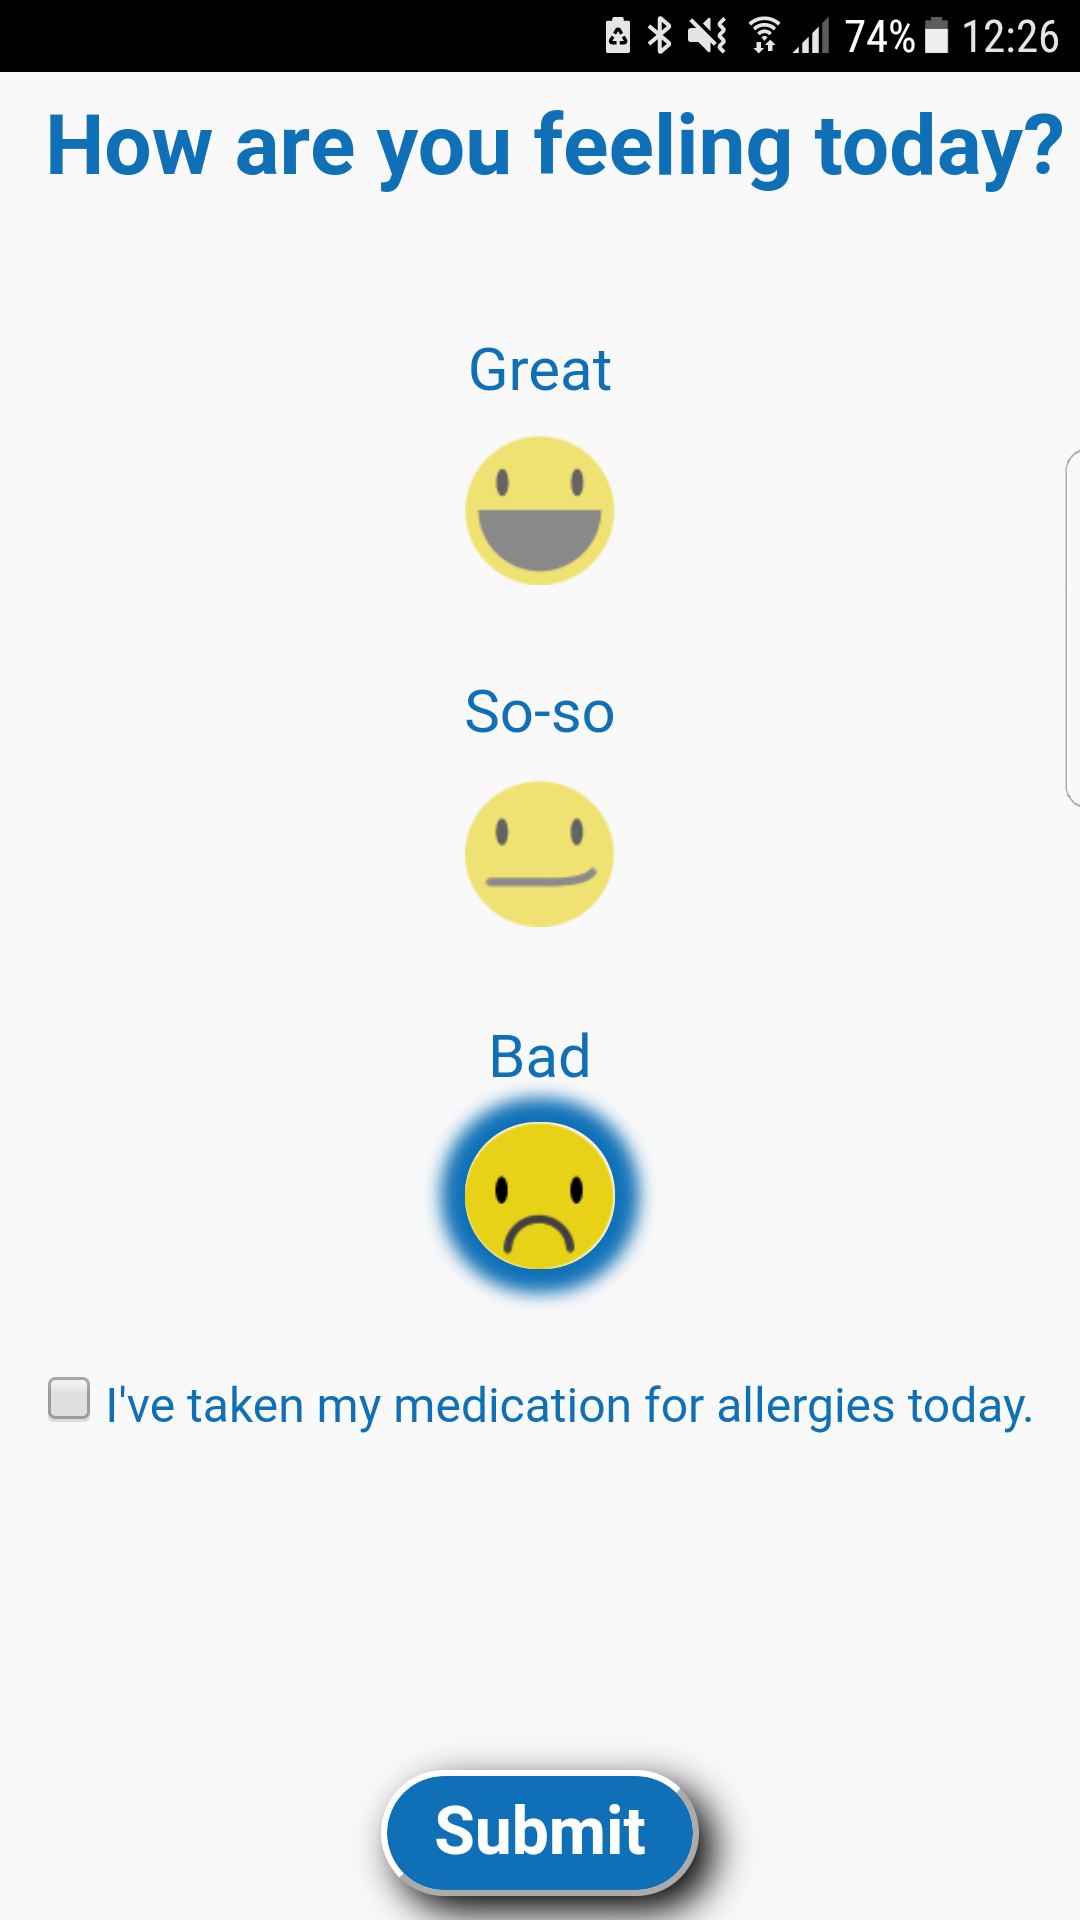
\includegraphics[width=6cm, height=8cm]{bbapp}
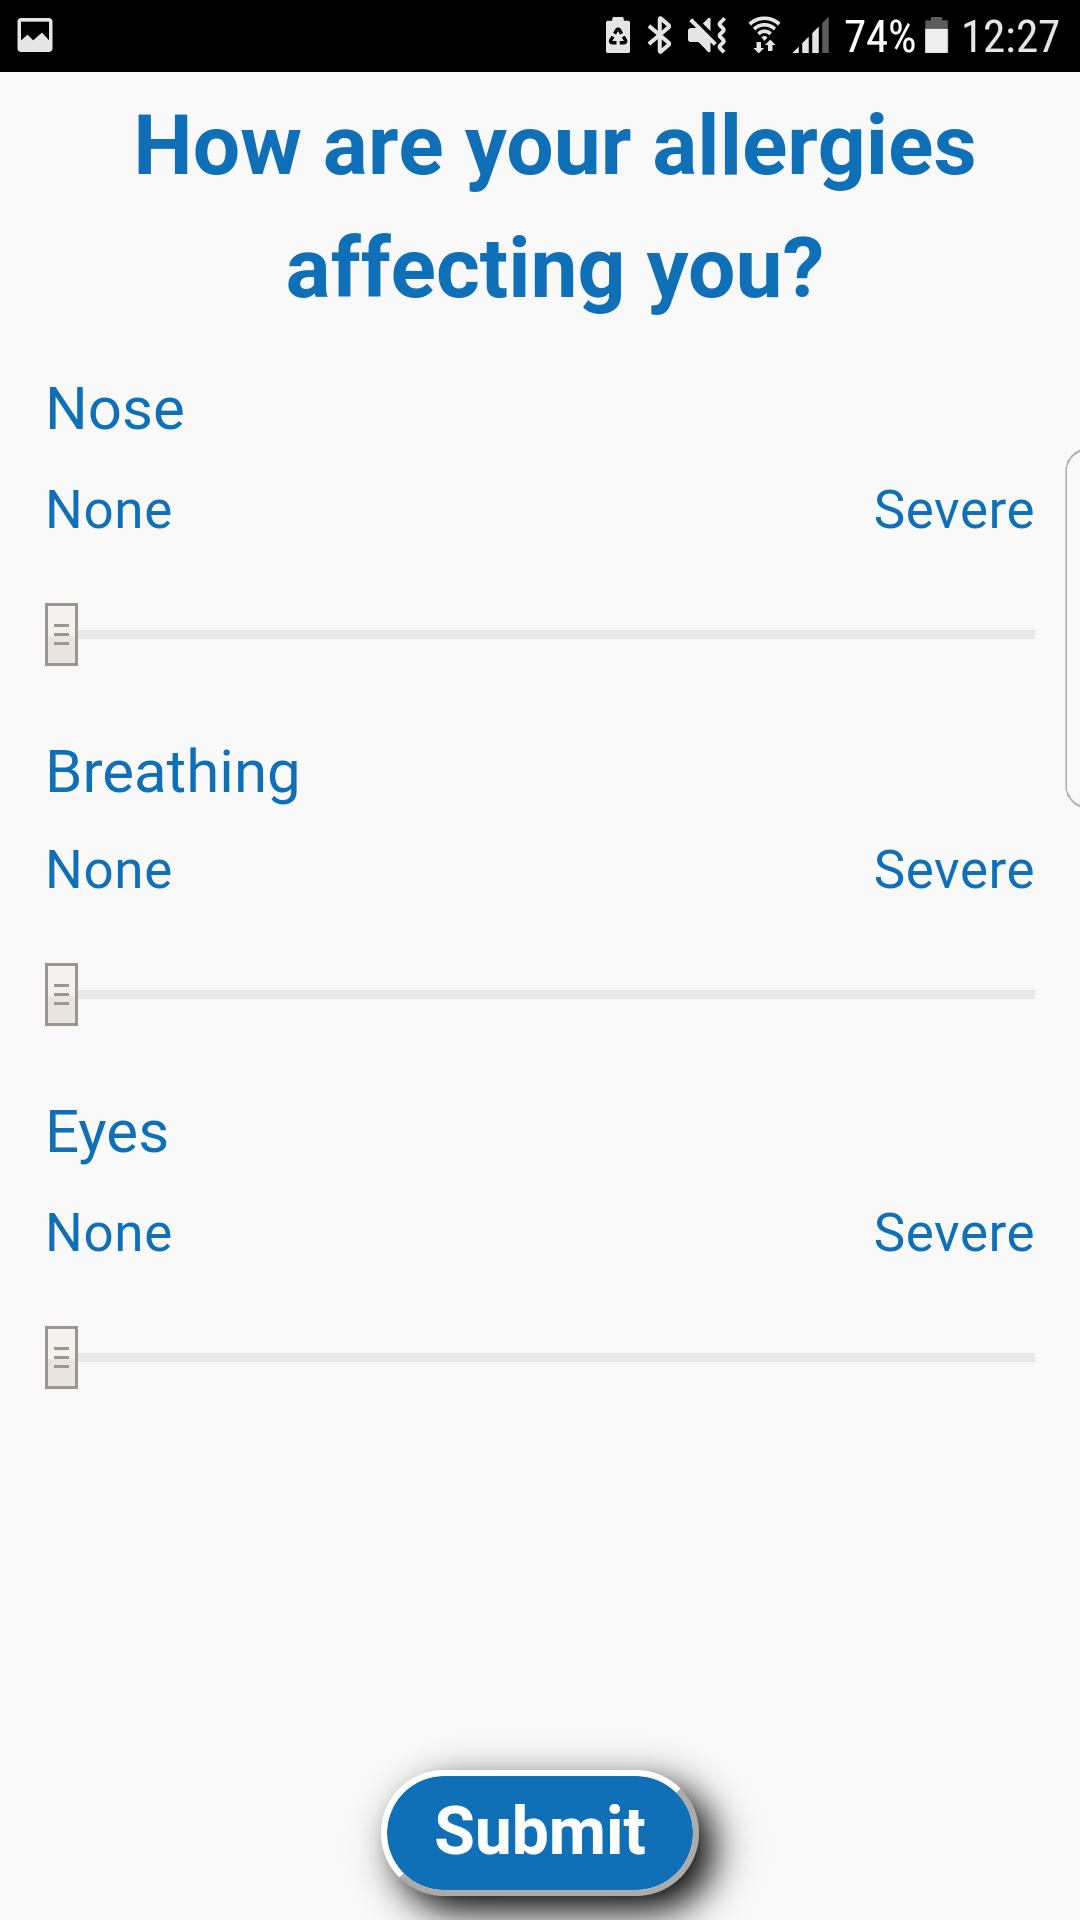
\includegraphics[width=6cm, height=8cm]{bbapp2}
\caption{Screenshots of the data collection screen on the Britain Breathing Android app}
\label{fig:bbscrn}
\end{center}
\end{figure}

Dr. Markel Vigo works with the Britain Breathing project and was kind enough to provide me with their dataset from September 2016. This dataset contains 18,386 records from all over the UK. The data contains values that attempt to measure the severity of certain symptoms such as how bad the users nasal symptoms are. They also ask whether or not the user has taken their medication today, this field is particularly useful as it can be used as a multiplier. If someone has severe nose, eye and breathing symptoms and they have taken their medication, then this should be represented in the final visualisation as they're obviously being exposed to a significant amount of allergens.\\

See \ref{bbdatatable} for an example of the data provided by Britain Breathing.

As the data contains many different symptom areas, I will have to focus my efforts on one particular problem. Trying to cover nose, eye and breathing problems would be too much for this project.


\begin{table}
\begin{center}
Britain Breathing Allergy Symptoms\\
\begin{tabular}{|c|c|c|c|c|c|c|c|c|c}\hline\hline
Breathing&Eyes&How Feeling&Nose&Taken Meds&Asthma&Hay Fever&Latitude&Longitude\\\hline
0&0&0&0&1&1&0&54.10&-2.39\\
3&0&2&3&1&1&1&53.89&-2.79\\
3&1&0&3&1&1&1&53.24&-2.34\\\hline\hline
\end{tabular}
\end{center}
\caption{Simplified example of the 18,386 record Britain Breathing dataset}\label{bbdatatable}
\end{table}

The Britain Breathing dataset will be the base for the entire project. Most of my time was spent with this set establishing a good hotspot identification algorithm.

\subsection{Other Datasets}

Whilst early testing and development involved many datasets, I decided on two main sets to use for the final version of Inhale.\\

The data.gov website has a road traffic count dataset available for public use. The set contains  750,000 entries for major road traffic counts at locations all over the UK. The sets give a location of the Centre Point of the count and for the northmost and southmost junctions on either side of the Centre Point. For each record, the counts for different vehicle types are given. Vehicles are categorised into Cars, Buses, Large Goods Vehicles (LGV), Heavy Goods Vehicle Rigid axle (HGVRx) where x is the number of axles of the HGVR.\\

See \ref{RoadTrafficData} for a simplified version of the dataset.\\

The second set used is the large urban areas in the UK. The data is fairly simple consisting of a location feature in the form of a Latitude and Longitude and a name for the area.\\


\begin{table}
\begin{center}
Road Traffic\\
\begin{tabular}{|c|c|c|c|c|c|c|c|c|c|c|}\hline\hline
S Ref E&S REF N&Road&A REF E&A REF N&Hour&CAR&BUS&LGV&HGVR2&...\\\hline
90200&10585&A3112&90320&10530&7&24&6&13&5&...\\
380927&405391&M60&382819&405920&15&7642&18&300&64&...\\
380927&405391&M60&382819&405920&17&10042&32&654&103&...\\\hline\hline
\end{tabular}

\caption{Simplified example of the 750,000 record Road Traffic dataset. 20 columns have been removed for viewing purposes.}\label{RoadTrafficData}
\end{center}
\end{table}

\section{Using Datasets}

The number of people suffering from allergic rhinitis is rising\cite{allergyrising}, and whilst increased carbon emissions are lengthening the pollen season \cite{co2pollen}, there are not significantly more pollen producing plants and trees year on year.\\

The main pollutants emitted by combustion engine vehicles are;\cite{vehcemis}

\begin{itemize}
    \item CO
    \item $SO_2$
    \item $NO_x$
\end{itemize}

It has been proven that these pollutants, whilst maybe not associated with hay fever symptoms by most, are actually all directly associated with allergic rhinitis\cite{airPollution}. With this in mind, we can compare the Road Traffic dataset with the Britain Breathing dataset on the same map to try to find some correlation.\\

\section{Existing Applications}
\label{sec:diagrams}

There are not many directly relevant applications. I think the reason for this is that in order to produce a meaningful application you need a well-formed dataset. In order for a dataset to be relevant, it needs to be of a reasonable size, have a good range of locations and a diverse demographic. Without collecting data from the people directly affected it's not going to be possible to make educated conclusions on allergy hotspots.\\

Looking at other applications did help highlight that I really was not a fan of using markers to represent any dense data.



\subsection{Britain Breathing}
Britain Breathing have a Data Visualiser on their website. It provides a simple display of the allergy data for a particular data range and a particular data value. At the time of writing this report, the Visualiser is not working so I can only display a screenshot of the interface and not the actual visualisation.

\begin{figure}[H]
\begin{center}
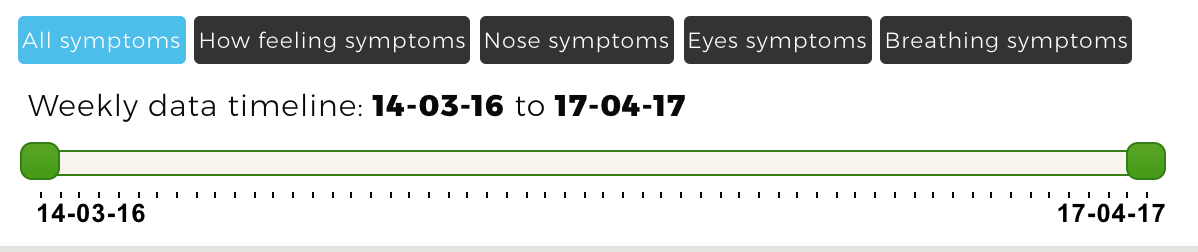
\includegraphics[width=0.75\textwidth]{bbvisinterface}
\caption{Figure Britain Breathing Visualiser Interface}
\end{center}
\end{figure}

\subsection{Pollen forecast}

The closest you can get to Inhale is pollen forecast services such as Pollen.com's Allergy forecast Map. As the name suggests it only shows the pollen forecasts, not allergy symptoms, and whilst this will have some correlation to the allergy symptoms, pollen is only a small part of the problem.\\

To get a good indication of allergy symptoms, unsurprisingly, you need allergy symptom data.\\

\begin{figure}[H]
\begin{center}
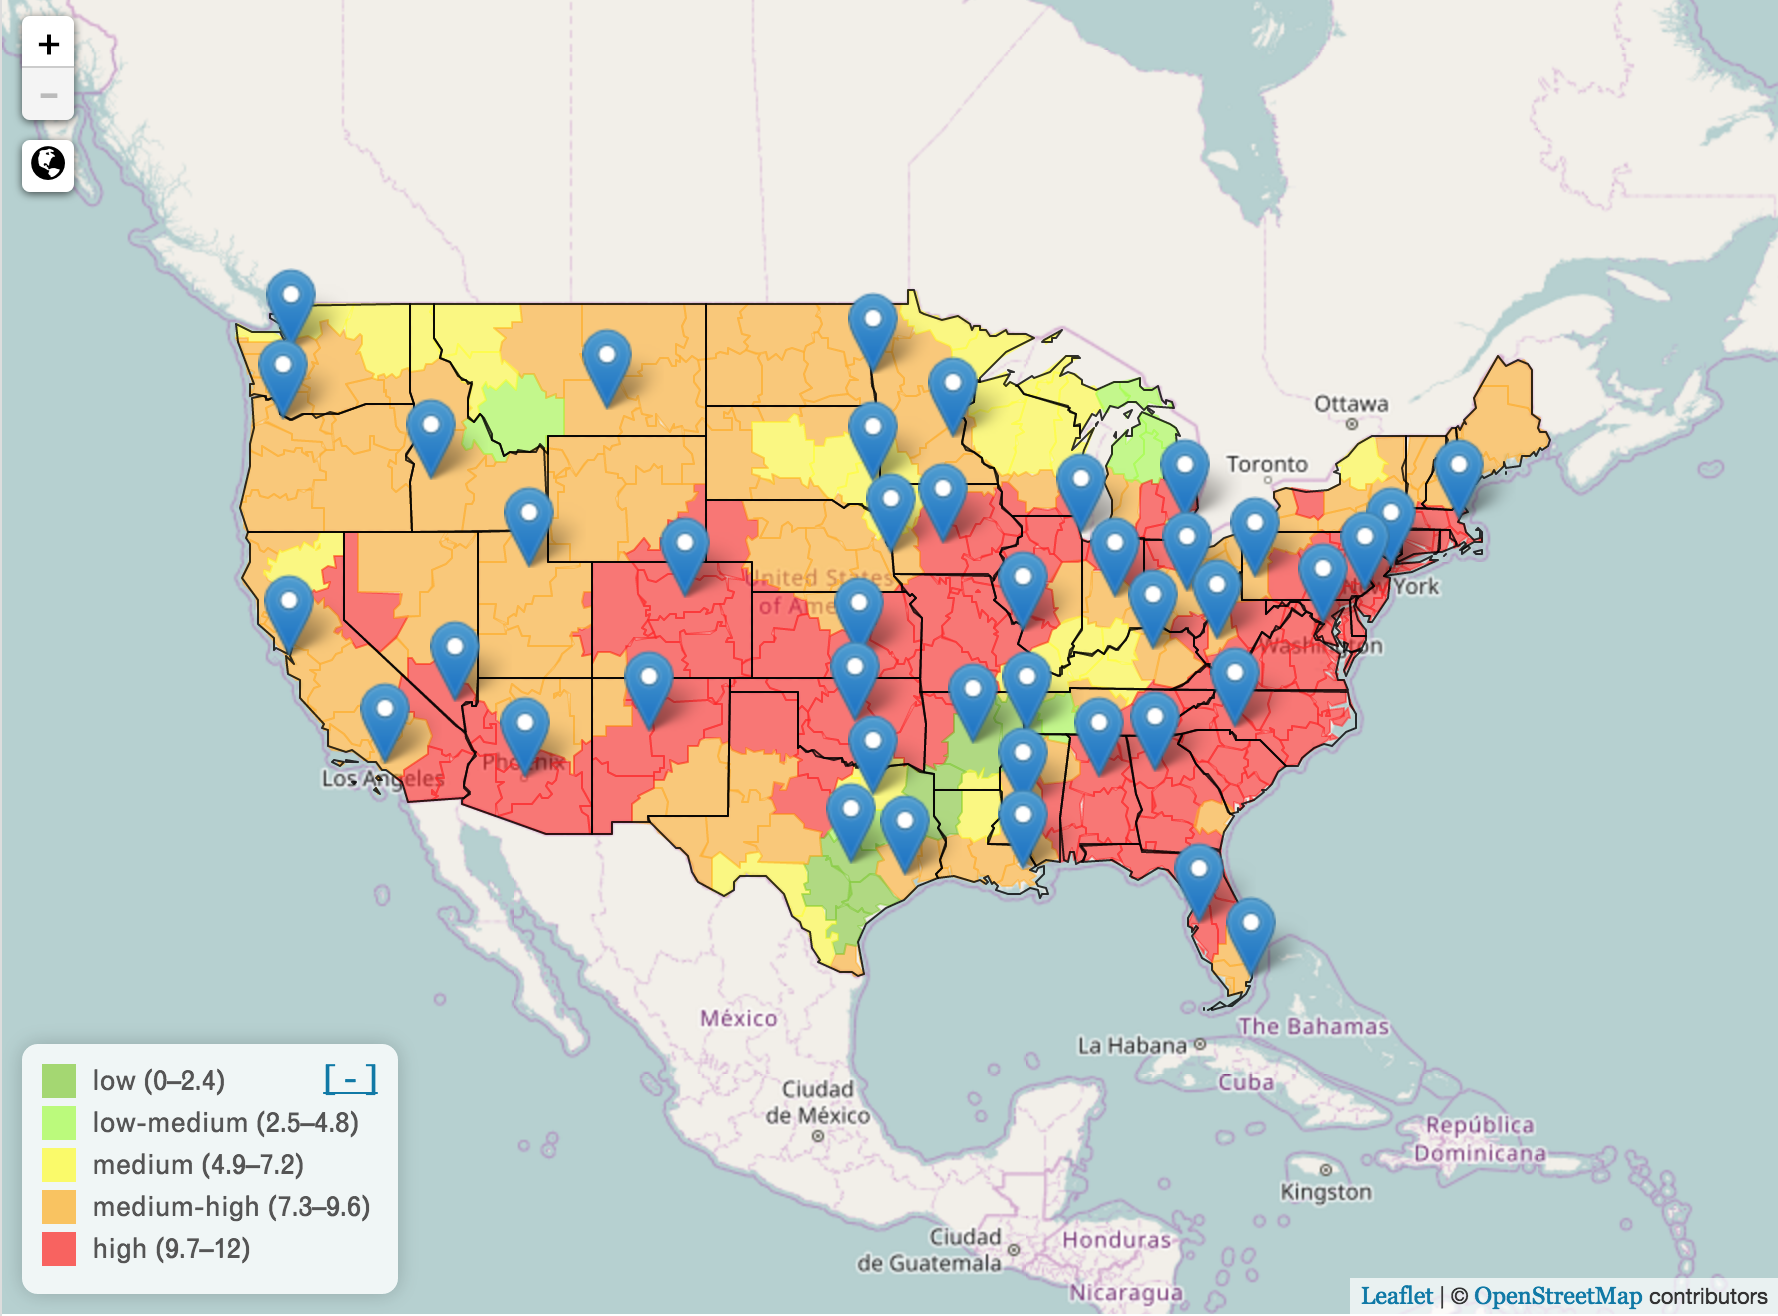
\includegraphics[width=0.75\textwidth]{pollenforecast}
\caption{Pollen.com Allergy Forecast Map}
\end{center}
\end{figure}